\documentclass[tikz,border=12pt]{standalone}
\usepackage[T1]{fontenc}
\usepackage{mathpazo}
\usepackage{amsmath,amssymb}
\usetikzlibrary{arrows.meta, positioning, calc}

\definecolor{stblue}{HTML}{7B97AD}
\definecolor{rwgold}{HTML}{B8995E}
\definecolor{sage}{HTML}{7A9A7E}
\definecolor{dkbrown}{HTML}{3D3530}
\definecolor{wmgray}{HTML}{7B7067}
\definecolor{cream}{HTML}{F9F6F0}
\definecolor{border}{HTML}{D4C9B8}
\definecolor{terracotta}{HTML}{C47A6A}
\definecolor{lavender}{HTML}{907EA0}

\begin{document}
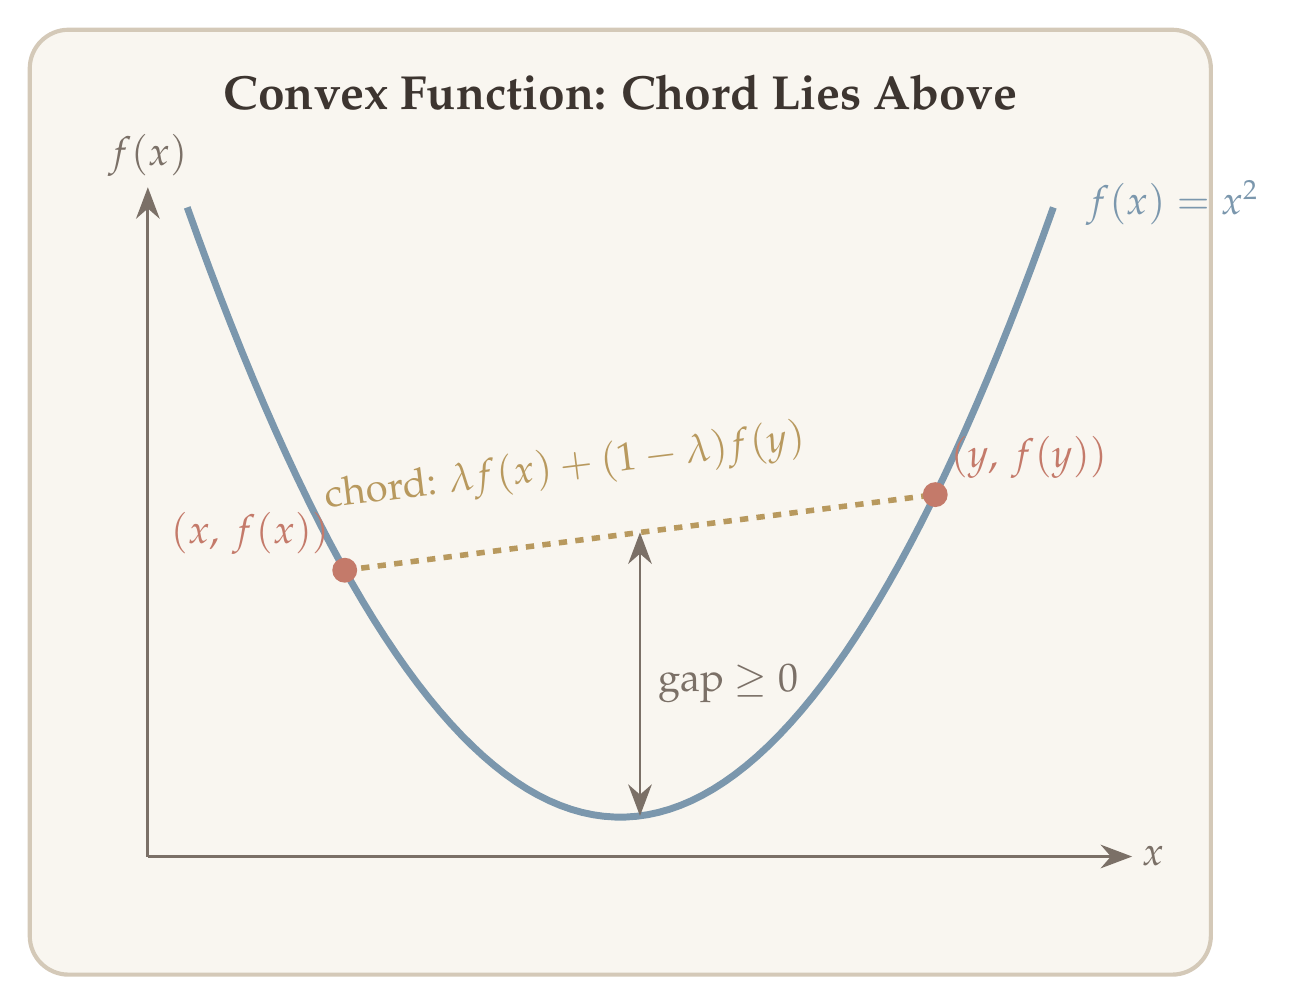
\begin{tikzpicture}[>={Stealth[length=4mm, width=3mm]}]

% Background — extra headroom for title, wider canvas
\fill[cream, rounded corners=14pt] (-0.5,-1.0) rectangle (14.5,11.0);
\draw[border, line width=1.5pt, rounded corners=14pt] (-0.5,-1.0) rectangle (14.5,11.0);

% Title — well above the plot area
\node[text=dkbrown, font=\LARGE\bfseries] at (7.0,10.2) {Convex Function: Chord Lies Above};

% Axes
\draw[wmgray, line width=1pt, ->] (1.0,0.5) -- (13.5,0.5) node[right, font=\Large, text=wmgray] {$x$};
\draw[wmgray, line width=1pt, ->] (1.0,0.5) -- (1.0,9.0) node[above, font=\Large, text=wmgray] {$f(x)$};

% Parabola f(x) = x^2, scaled wider
% Parametric: real x from -2.2 to 2.2, canvas x = 7.0 + 2.5*real_x, canvas y = 1.0 + 1.6*real_x^2
\draw[stblue, line width=2.5pt, domain=-2.2:2.2, samples=80]
  plot ({7.0 + 2.5*\x}, {1.0 + 1.6*\x*\x});
\node[text=stblue, font=\Large, right] at (12.8,8.8) {$f(x) = x^2$};

% Points: x1 at real -1.4, x2 at real 1.6
% Canvas: x1 = 7.0 + 2.5*(-1.4) = 3.5,  y1 = 1.0 + 1.6*1.96 = 4.136
%         x2 = 7.0 + 2.5*(1.6) = 11.0,   y2 = 1.0 + 1.6*2.56 = 5.096
\coordinate (P1) at (3.5, 4.136);
\coordinate (P2) at (11.0, 5.096);

% Chord (dashed)
\draw[rwgold, line width=2pt, dashed] (P1) -- (P2);

% Points
\fill[terracotta] (P1) circle (4.5pt);
\fill[terracotta] (P2) circle (4.5pt);

% Labels
\node[text=terracotta, font=\Large, above left=3pt] at (P1) {$(x,\, f(x))$};
\node[text=terracotta, font=\Large, above right=3pt] at (P2) {$(y,\, f(y))$};

% Chord label — shifted left to avoid overlap with (y, f(y))
\node[text=rwgold, font=\Large, above=4pt, rotate=7] at ($(P1)!0.38!(P2)+(0,0.4)$)
  {chord: $\lambda f(x) + (1-\lambda) f(y)$};

% Annotation: chord >= function
% Function value at midpoint real x = (-1.4+1.6)/2 = 0.1, canvas x = 7.25, y = 1.0+1.6*0.01 = 1.016
% Chord at canvas x=7.25: 4.136 + (5.096-4.136)*((7.25-3.5)/(11.0-3.5))
\draw[wmgray, line width=1pt, <->] (7.25,{1.0+1.6*0.01}) -- (7.25,{4.136 + (5.096-4.136)*((7.25-3.5)/(11.0-3.5))});
\node[text=wmgray, font=\Large, right=3pt] at (7.25,2.7) {gap $\geq 0$};

\end{tikzpicture}
\end{document}
